\chapter{Contribuição}
\label{cap_contribuicao}

Nesta secção, será relatado o trabalho realizado no intuito da componente prática do projeto e os resultados. 
% Neste caso, relevante à criação de um \textit{toolkit} e ferramentas para a extração do conteúdo de documentos antigos, em particular jornais, com melhores resultados do que os oferecidos pelas ferramentas de \acrshort{ocr} base e, possibilitando a obtenção da lógica e organização original dos mesmos.

\section{Introdução}
% Ao longo do período de inicialização da dissertação: desde a definição dos objetivos do projeto, aprofundamento da temática e estudo do estado da arte; de forma a simultaneamente acostumar com as tecnologias, assim como ganhar um melhor entendimento sobre os algoritmos a implementar e os desafios apresentados, algum trabalho prático já foi realizado. 
% Este envolve principalmente a criação de uma ferramenta para facilitar a visualização dos resultados de reconhecimento, assim como o debugging destes e alguns algoritmos preliminares para manipulação destes resultados de \acrshort{ocr}.

A discussão sobre o trabalho realizado será estruturada em 3 componentes principais.
\begin{itemize}
	\item Ferramentas do \textit{toolkit} desenvolvidas \ref{contribution_toolkit}
	\item Pipeline de aplicação do toolkit \ref{contribution_toolkit_pipeline}
% 	\item GUI de aplicação geral do \textit{toolkit}
	\item GUI editor OCR \ref{contribution_ocr_editor}
\end{itemize}

Para cada uma das secções delimitadas, será dada uma explicação do seu propósito e produto sumariado, procedido por uma discussão mais detalhada dos elementos que a constituem.

De forma geral, o código desenvolvido foi maioritariamente escrito em Python, com algumas instâncias de C.

\section{Ferramentas do \textit{toolkit} desenvolvidas}
\label{contribution_toolkit}

\subsection{Introdução}

A componente do \textit{toolkit} foi a premissa base do tema da dissertação. Um conjunto de ferramentas focado na melhoria dos resultados obtidos da aplicação de \acrshort{ocr} em documentos antigos, com especial interesse em jornais. 

Estas ferramentas são então pertinentes para os diversos passos do processo convencional de \acrshort{ocr}, i.e. pré-processamento, OCR e pós-processamento; atendendo tanto a processamento de imagem, processamento de resultados de OCR e texto, e validação de resultados.

Além dos métodos principais criados para a resolução de problemas identificados, é importante realçar certos pontos essenciais que serviram como base para o resto do trabalho. Estes são as estruturas de dados utilizadas para o tratamento dos resultados de OCR.

\subsection{Sumário}

\begin{itemize}\setlength\itemsep{-0.3em}
	\item Estruturas de dados \ref{data_structures}
	\begin{itemize}\setlength\itemsep{-0.3em}
		\item OCR Tree \ref{ocr_tree}
		\item Box \ref{box_data_structure}
	\end{itemize}
	\item Métodos \ref{contribution_methods}
	
	\begin{itemize}\setlength\itemsep{-0.3em}
		\item Processamento de resultados OCR \ref{contribution_ocr_posprocessing}
		
		\begin{itemize}\setlength\itemsep{-0.3em}
			\item Conversão de resultados OCR \ref{ocr_results_conversion}
			\item Debugging \ref{contribution_debugging}
			\item Análise de texto \ref{contribution_text_analyses}
			\item Limpeza de OCR Tree \ref{contribution_clean_ocr}
			\item Categorização de Blocos \ref{contribution_categorize_blocks}
			\item Divisão de blocos \ref{contribution_divide_blocks}
			\item Cálculo de ordem de leitura \ref{contribution_reading_order}
			\item Segmentação de resultados \ref{contribution_result_segmentation}
		\end{itemize}
		
		\item Processamento de imagem \ref{contribution_image_processing}
		\begin{itemize}\setlength\itemsep{-0.3em}
			\item Binarização de imagem
			\item Rotação de imagem
			\item Cálculo de sentido de rotação
			\item Segmentação de documento
			\item Identificação de imagens
			\item Identificação de delimitadores
			\item Divisão de colunas 
		\end{itemize}
		
		\item Processamento de texto \ref{contribution_text_processing}
		\begin{itemize}\setlength\itemsep{-0.3em}
			\item Limpeza de hifenização
		\end{itemize}
		
	\end{itemize}
	
	\item Validação de resultados \ref{contribution_results_validation}
	
\end{itemize}


\subsection{Estruturas de dados}
\label{data_structures}


\subsubsection{OCR Tree}
\label{ocr_tree}

Como o produto final do projeto intende aceitar diferentes tipos de resultados OCR, i.e. resultantes de diferentes motores OCR ou de ficheiros como hOCR que já possuem os resultados, existe uma necessidade de converter estes diferentes formatos num único tipo que mantenha a informação base pretendida.

Estruturas de dados standard como \citep{hocr_doc} ou \citep{alto_doc} apresentam um resultado final semelhante e com capacidade base de armazenamento de meta-dados superior porém, sendo baseados em XML, tornam a sua manipulação mais complexa e, em múltiplos casos a informação proporcionada é além do necessário ou gera conclusões erradas quando gerado de output automático (ex.: atribuição de classes caption a blocos que são títulos). Assim sendo, embora tenha sido desenvolvido um conversor de, e para HOCR, para o atual projeto, optou-se pela criação de uma estrutura de dados própria.

Deste modo, tomando como inspiração os atributos dos resultados do Tesseract no modo de dicionário \citep{tesseract_doc}, foi implementada uma estrutura de dados no formato de árvore de dados.

A escolha de uma estrutura de árvore permite a hierarquização de blocos de acordo com o seu nível, quer exista uma divisão de nível à partida, como é o caso do Tesseract que segue: página $\longrightarrow$ bloco $\longrightarrow$ parágrafo $\longrightarrow$ linha $\longrightarrow$ palavra; ou apenas um único nível, semelhante ao Keras-OCR.

Todos os algoritmos desenvolvidos, inclusive os métodos para visualização (métodos de debugging e GUI desenvolvido), assumem e trabalham com os dados de OCR no formato desta estrutura de dados.

As características mais relevantes desta estrutura são:

\begin{itemize}\setlength\itemsep{-0.3em}
	\item \textbf{Level} : Nível/altura do nodo.
	\begin{itemize}\setlength\itemsep{-0.3em}
		\item documento : 0
		\item página 	: 1
		\item bloco		: 2
		\item parágrafo : 3
		\item linha 	: 4
		\item palavra	: 5
	\end{itemize}\setlength\itemsep{-0.3em}
	\item \textbf{(page|block|par|line|word)\_num}: Identificação da ordem (dentro de outras caixas(ex.: linha), se aplicável)
	\item \textbf{text} : Texto do bloco, normalmente apenas preenchido ao nível da palavra
	\item \textbf{conf} : Confiança no texto
	\item \textbf{id}
	\item \textbf{type} : Tipo do bloco, ex.: delimitador, título
	\item \textbf{children}
	\item \textbf{box}: Bounding box do nodo, representado pela estrutura de dados Box, que também possui métodos para transformações e verificações geométricas ou de características.
	\item Características de texto: ex.: texto iniciado (start\_text); texto não terminado (end\_text).
\end{itemize}

%% TODO : Ilustracao de uso de arvore OCR para demonstrar diferentes niveis de um documento

Construtores da classe são capazes de admitir outros atributos não base de modo a expandir a utilidade da estrutura. Construtores disponíveis: iniciação por argumentos, dicionário, ficheiro JSON e ficheiro HOCR.

Da mesma forma, conversores para estes ficheiros compreendidos para iniciação também foram desenvolvidos.

A classe possuí por métodos de transformação e análise sobre a árvore OCR que facilitam a manipulação dos resultados OCR. 

Segue-se uma lista dos métodos mais relevantes disponíveis da classe.

\highlight{id\_boxes}
 
 
\textbf{Descrição:} Adiciona identificador aos blocos.
	
\textbf{Argumentos:}
	\begin{itemize}\setlength\itemsep{-0.3em}
		\item level : lista de níveis onde adicionar identificador
		\item ids (opt): dicionário de ids a utilizar caso não se queira iniciar no 0.
		\item delimiters (opt): flag para identificar delimitadores
		\item area (opt): argumento do tipo Box, que restringe os nodos a identificar a uma dada área
		\item override (opt): flag para reescrever id se já existe.
	\end{itemize}
				
\highlight{calculate\_mean\_height}

\textbf{Descrição:} Calcula a altura média das caixas de um dado nível.
	
\textbf{Argumentos:}
\begin{itemize}\setlength\itemsep{-0.3em}
	\item level : nível a calcular
	\item conf (opt): valor de confiança de texto no caso de apenas serem relevantes caixas com certa confiança (aplicável apenas para nível de texto)
\end{itemize}

	
\highlight{is\_text\_size}

\textbf{Descrição:} Verifica se um nodo se encontra dentro do tamanho de texto.
	
\textbf{Argumentos:}
\begin{itemize}\setlength\itemsep{-0.3em}
	\item text\_size : tamanho de texto a comparar
	\item mean\_height (opt): altura do bloco, caso já tenha sido calculado
	\item range : margem de erro aceitável (relativo)
	\item level : nível das caixas usado caso seja necessário calcular a altura média
	\item conf : confiança do texto a utilizar para calcular a altura média
\end{itemize}

\highlight{is\_empty}

\textbf{Descrição:} Verifica se um nodo é vazio.
	
\textbf{Argumentos:}
\begin{itemize}\setlength\itemsep{-0.3em}
	\item conf : confiança de texto a utilizar para considerar palavras válidas
	\item only\_text : flag que dita se o tipo do bloco influencia o resultado, i.e. blocos de tipo "image" não são vazios
\end{itemize}

	
\highlight{text\_is\_title}

\textbf{Descrição:} Verifica se um nodo é potencial título.
	
\textbf{Algoritmo:} Caixa não é texto vertical e é maior do que o tamanho normal de texto.


\textbf{Argumentos:}
\begin{itemize}\setlength\itemsep{-0.3em}
	\item normal\_text\_size : tamanho de texto considerado como normal
	\item conf : confiança de texto a utilizar para considerar palavras válidas
	\item range : margem de acerto aceitável (relativo)
	\item level : nível usado para calcular o tamanho médio do bloco
\end{itemize}

	
\highlight{is\_delimiter}

\textbf{Descrição:} Verifica se um nodo é potencial delimitador.
	
\textbf{Algoritmo:} Caixa já é do tipo delimitador, ou é vazia e segue a regra:

$ box.width >= box.height*4 || box.height >= box.widht*4 $.


\textbf{Argumentos:}
\begin{itemize}\setlength\itemsep{-0.3em}
	\item conf : confiança de texto a utilizar para considerar palavras válidas
	\item only\_type : flag que dita se usa apenas o tipo do nodo para a verificação
\end{itemize}

	
\highlight{is\_image}

\textbf{Descrição:} Verifica se um nodo é potencial imagem.
	
\textbf{Algoritmo:} Caixa já é do tipo imagem ou, é vazia, não é um delimitador e é 3 vezes mais alta do que o tamanho de texto.


\textbf{Argumentos:}
\begin{itemize}\setlength\itemsep{-0.3em}
	\item conf : confiança de texto a utilizar para considerar palavras válidas
	\item text\_size : tamanho de texto a utilizar para comparação com altura da caixa
	\item only\_type : flag que dita se usa apenas o tipo do nodo para a verificação
\end{itemize}


\highlight{get\_boxes\_in\_area}

\textbf{Descrição:} Obtém todas as caixas numa dada área.


\textbf{Argumentos:}
\begin{itemize}\setlength\itemsep{-0.3em}
	\item area : área de interesse
	\item level : nível dos nodos a ir buscas. Se nível == -1, obtém todos os nodos
	\item conf : confiança de texto a utilizar para considerar nodos válidos
	\item ignore\_type : tipos de nodo a ignorar
\end{itemize}
	
	
\highlight{is\_vertical\_text}

\textbf{Descrição:} Verifica se um nodo é texto vertical.

\textbf{Argumentos:}
\begin{itemize}\setlength\itemsep{-0.3em}
	\item conf : confiança de texto a utilizar para considerar palavras válidas
\end{itemize}
	
\textbf{Algoritmo:}

\begin{algorithm}[H]
	\caption{Verificação de texto vertical}
	\algsetup{linenosize=\tiny}
	\tiny
	\begin{algorithmic}[1]
		\IF{nodo não é vazio}
			\STATE lines
			\IF{len(lines) == 0}
				\RETURN False
			\ENDIF
			\STATE \textit{// Linha única}
			\IF{len(lines) == 1}
				\STATE words
			 \STATE \textit{// Palavra única}
				\IF{len(words) == 1}
					\IF{altura da palavra >= 2 * largura da palavra}
						\RETURN True
					\ENDIF
				\STATE \textit{// Múltiplas palavras} 
				
				\Else
					\STATE \textit{// Verifica se a maioria das palavras coincidem horizontalmente}
					\STATE widest\_word <- calcula palavra mais larga
					\STATE overlapped\_words = 0
					\FOR{word in words}
						\IF{word == widest\_word}
							\STATE continue
						\ENDIF
						\IF{word.box.within\_horizontal\_boxes(widest\_word.box,range=0.1)}
							\STATE overlapped\_words += 1
						\ENDIF
					\ENDFOR
					\IF{overlapped\_words/len(words) >= 0.5}
						\RETURN True
					\ENDIF
					
				\ENDIF
				
			\STATE \textit{// Múltiplas linhas} 
			
			\Else
				\STATE \textit{// Verifica se a maioria das linhas coincidem verticalmente}
				\STATE tallest\_line <- calcula linha mais alta
				\STATE overlapped\_lines = 0
				
				\FOR{line in lines}
					\IF{line == tallest\_line}
						\STATE continue
					\ENDIF
					\IF{line.box.withinvertical\_boxes(tallest\_line.box,range=0.1)}
						\STATE overlapped\_lines += 1
					\ENDIF
				\ENDFOR
				\IF{overlapped\_lines/len(lines) >= 0.5}
					\RETURN True
				\ENDIF
			
			\ENDIF
			
		\ENDIF
		
		\RETURN	False
		
	\end{algorithmic}
\end{algorithm}



\highlight{prune\_children\_area}

\textbf{Descrição:} Atualiza dimensões dos filhos de um nodo para se encaixarem dentro de uma área.


\textbf{Argumentos:}
\begin{itemize}\setlength\itemsep{-0.3em}
	\item area : área de interesse
\end{itemize}


\highlight{boxes\_below}
(método semelhante para as outras direções)

\textbf{Descrição:} Dada uma lista de OCR Tree, devolve aqueles que se encontram por baixo do bloco atual. Os blocos filtrados podem intersetar ou estar dentro do bloco comparado.


\textbf{Argumentos:}
\begin{itemize}\setlength\itemsep{-0.3em}
	\item blocks : lista de blocos a filtrar
\end{itemize}



\highlight{boxes\_directly\_below}
(método semelhante para as outras direções)

\textbf{Descrição:} Dada uma lista de OCR Tree, devolve aqueles que se encontram diretamente por baixo do bloco atual. Blocos filtrados não estão dentro do bloco comparado e não podem estar diretamente por baixo dos outros blocos.


\textbf{Argumentos:}
\begin{itemize}\setlength\itemsep{-0.3em}
	\item blocks : lista de blocos a filtrar
\end{itemize}
	
	
	
\highlight{join\_trees}

\textbf{Descrição:} Junta duas OCR Tree com do mesmo nível numa única árvore. Tem dois métodos principais de junção das árvores: vertical, operação mais simples em que basicamente apenas se juntam as duas listas de ramos dos nodos raíz (assume-se que uma das árvores é mais alta do que a outra e não se intersetam); e horizontal, onde se procura juntar árvores que têm interseção no eixo y, sendo necessário verificar as posições que os filhos devem tomar e se certos filhos devem ser unidos num único (podendo resultar numa junção de linhas).

%% TODO : ilustração poderá ajudar


\textbf{Argumentos:}
\begin{itemize}\setlength\itemsep{-0.3em}
	\item tree : árvore a juntar
	\item orientation : orientação da junção, vertical ou horizontal.
\end{itemize}

\textbf{Algoritmo:}

\begin{algorithm}[H]
	\caption{Junção horizontal}
	\algsetup{linenosize=\tiny}
	\tiny
	\begin{algorithmic}[1]
		\STATE tree\_children
		\STATE self\_children
		\STATE \textit{// no último nível, filhos são ordenados da esquerda para a direita}
		\IF{último nível da tree}
			\STATE tree\_children $\leftarrow$ ordenar lista da esquerda para a direita
		\ENDIF
		
		\FOR{child in tree\_children}
			\IF{não é o último nível}
				\STATE self\_children $\leftarrow$ ordena de cima para baixo
				\IF{child pode ser inserida no topo ou fundo da lista}
					\STATE self\_children $\leftarrow$ insere child no início ou fim
				\ELSE
					\STATE \textit{// procura slot para inserir, ou nodo com quem unir}
					\STATE joined = False
					\FOR{i in range(len(self\_children))}
						\IF{child não interseta com nodo i ou nodo i+1}
							\STATE self.children $\leftarrow$ adiciona child entre os dois nodos
							\STATE joined = True
						\ELSIF{interseta com nodo i}
							\IF{interseção em pelo menos 70\% da altura da caixa}
								\IF{nodo i tem filhos}
									\STATE \textit{// join recursivo}
									\STATE self\_children[i].join\_trees(child,orientation=orientation)
								\ELSE
									\STATE self\_children $\leftarrow$ insere child depois do nodo i
								\ENDIF
								\STATE joined = True
							\ELSE
								\STATE \textit{// procura local mais baixo para inserir (por poder intersetar com varios blocos)}
								\FOR{j in range(i,len(self\_children))}
									\IF{nodo j mais alto do que child}
										\STATE self\_children $\leftarrow$ insere child depois do nodo j
										\STATE joined = True
									\ENDIF
								\ENDFOR
								\IF{not joined}
									\STATE self\_children $\leftarrow$ insere child no fim
									\STATE joined = True
								\ENDIF
							\ENDIF
						\ENDIF
						
						\IF{joined}
							\STATE break
						\ENDIF
					\ENDFOR
				\ENDIF
			\ELSE
				\STATE self.children $\leftarrow$ adiciona child no fim da lista
			\ENDIF
			
			\STATE self\_children $\leftarrow$ atualiza lista de filhos
		\ENDFOR
		
		
	\end{algorithmic}
\end{algorithm}


\highlight{remove\_blocks\_inside}

\textbf{Descrição:} Remove os blocos dentro do bloco com dado id. Blocos removidos são do mesmo nível que o bloco com dado id.


\textbf{Argumentos:}
\begin{itemize}\setlength\itemsep{-0.3em}
	\item id : id do bloco a limpar
	\item block\_level : nível do bloco a limpar
\end{itemize}

\highlight{update\_position}

\textbf{Descrição:} Atualiza a posição da bounding box de um nodo e dos seus filhos. Especialmente útil para o editor OCR.


\textbf{Argumentos:}
\begin{itemize}\setlength\itemsep{-0.3em}
	\item top : valor a atualizar verticalmente
	\item left : valor a atualizar horizontalmente
	\item absolute : flag que indica se operação é de do tipo absoluta, i.e. bounding box vai ser diretamente atualizada com estes valores, ou relativa, aos valores da bounding box serão somados os argumentos
\end{itemize}

\highlight{update\_size}

\textbf{Descrição:} Atualiza o tamanho da bounding box de um nodo e dos seus filhos nas arestas (filhos interiores não serão alterados). Especialmente útil para o editor OCR.


\textbf{Argumentos:}
\begin{itemize}\setlength\itemsep{-0.3em}
	\item top : valor a atualizar ao topo
	\item left : valor a atualizar à esquerda
	\item bottom : valor a atualizar ao fundo
	\item right : valor a atualizar à direita
	\item absolute : flag que indica se operação é de do tipo absoluta, i.e. bounding box vai ser diretamente atualizada com estes valores, ou relativa, aos valores da bounding box serão somados os argumentos
\end{itemize}

\highlight{update\_box}

\textbf{Descrição:} Atualiza diretamente valor da bounding box do nodo e dos filhos. Especialmente útil para o editor OCR.

\textbf{Argumentos:}
\begin{itemize}\setlength\itemsep{-0.3em}
	\item top : valor a atualizar ao topo
	\item left : valor a atualizar à esquerda
	\item bottom : valor a atualizar ao fundo
	\item right : valor a atualizar à direita
	\item children : flag que indica se é para se aplicar ajuste direto no nodo, ou apenas ajustar de forma a não sair da bounding box do pai.
\end{itemize}

\highlight{scale\_dimensions}

\textbf{Descrição:} Escala dimensões da bounding box do nodo e dos seus filhos. Especialmente útil para o editor OCR.

\textbf{Argumentos:}
\begin{itemize}\setlength\itemsep{-0.3em}
	\item scale\_width : escalar de valores do eixo horizontal
	\item scale\_height : escalar de valores do eixo vertical
\end{itemize}


\subsubsection{Box}
\label{box_data_structure}

A estrutura de dados Box é utilizada maioritariamente para encapsular os dados das bounding boxes dos resultados de OCR. Embora em geral este tipo de dados seja geralmente fornecido por métodos de módulos de manipulação de imagens na forma de tuplo, a utilização de uma classe dedicada permite o desenvolvimento e utilização de métodos para sua manipulação de forma mais simples e organizada.

Tal como a estrutura de dados OCR Tree, esta classe apresenta construtores e conversores de ficheiros diferentes tipos: argumentos simples, dicionário, ficheiro JSON.

Os principais atributos da estrutura são:

\begin{itemize}\setlength\itemsep{-0.3em}
	\item \textbf{left} 	: Valor mais à esquerda da caixa.
	\item \textbf{right}	: Valor mais à direita da caixa.
	\item \textbf{top} 		: Valor mais em cima da caixa (menor do que bottom por ser baseado em manipulação de imagem). 
	\item \textbf{bottom} 	: Valor mais em baixo da caixa.
	\item \textbf{width} 	: Comprimento da caixa.
	\item \textbf{height} 	: Altura da caixa.
\end{itemize}

Realça-se que os atributos desta classe são esperados no formato de inteiros, devido a ter como foco o seu uso no contexto do espaço de imagens.

Segue-se uma lista dos métodos mais relevantes disponíveis da classe.

\highlight{update}

\textbf{Descrição:} Atualiza os valores dos atributos de posição da caixa. Atributos de posição são mantidos válidos, i.e. left <= right e top <= bottom . Altura e comprimento são atualizados automaticamente.

\textbf{Argumentos:}
\begin{itemize}\setlength\itemsep{-0.3em}
	\item top : valor a atualizar ao topo
	\item left : valor a atualizar à esquerda
	\item bottom : valor a atualizar ao fundo
	\item right : valor a atualizar à direita
\end{itemize}


\highlight{move}

\textbf{Descrição:} Soma valores aos atributos de posição da caixa.

\textbf{Argumentos:}
\begin{itemize}\setlength\itemsep{-0.3em}
	\item x : valor a somar nos atributos de posição horizontais
	\item y : valor a somar nos atributos de posição verticais
\end{itemize}

\highlight{within\_vertical\_boxes}
(método semelhante para direção horizontal)

\textbf{Descrição:} Verifica se caixa e caixa a ser comparada estão alinhadas verticalmente, podendo considerar uma margem de acerto. Verificação é realizada nos dois sentidos, i.e. caixa 1 alinhada com caixa 2 ou vice-versa.

\textbf{Argumentos:}
\begin{itemize}\setlength\itemsep{-0.3em}
	\item box : caixa a comparar
	\item range : valor relativo da altura da caixa, a servir como margem para considerar na verificação
\end{itemize}

\highlight{is\_inside\_box}

\textbf{Descrição:} Verifica se caixa a ser comparada está dentro da caixa. Caixa a ser compara tem de estar completamente dentro para resultado afirmativo.

\textbf{Argumentos:}
\begin{itemize}\setlength\itemsep{-0.3em}
	\item box : caixa a comparar
\end{itemize}


\highlight{intersects\_box}

\textbf{Descrição:} Verifica se caixa a ser comparada interseta com a caixa.

\textbf{Argumentos:}
\begin{itemize}\setlength\itemsep{-0.3em}
	\item box : caixa a comparar
	\item extend\_vertical : flag para indicar se verificação deve ser feita apenas longo do eixo x (ex.: utilizado para verificar se caixa comparada está diretamente por acima da caixa)
	\item extend\_horizontal : flag para indicar se verificação deve ser feita apenas longo do eixo y (ex.: utilizado para verificar se caixa comparada está diretamente à direita caixa)
	\item inside : flag para indicar se verificação de caixa dentro conta como interseção
\end{itemize}


\highlight{intersect\_area\_box}

\textbf{Descrição:} Calcula a caixa de interseção entre a caixa e uma caixa a comparar.

\textbf{Argumentos:}
\begin{itemize}\setlength\itemsep{-0.3em}
	\item box : caixa a comparar
\end{itemize}


\highlight{remove\_box\_area}

\textbf{Descrição:} Remove área da caixa. Procura remover área aplicando as menores modificações possíveis. Apenas realiza modificações, se área fornecida está dentro da caixa.

\textbf{Argumentos:}
\begin{itemize}\setlength\itemsep{-0.3em}
	\item area : area da caixa a remover
\end{itemize}


\highlight{get\_box\_orientation}

\textbf{Descrição:} Método naive para obter orientação da caixa (horizontal, vertical ou square) de acordo com a diferença entre a sua altura e comprimento.


\highlight{join}

\textbf{Descrição:} Une duas caixas.

\textbf{Argumentos:}
\begin{itemize}\setlength\itemsep{-0.3em}
	\item box : caixa a unir
\end{itemize}

\highlight{distance\_to}

\textbf{Descrição:} Calcula distância entre duas caixas. Procura dois pontos mais próximos de acordo com argumentos dados e utiliza distância euclidiana para calcular a distância.

\textbf{Argumentos:}
\begin{itemize}\setlength\itemsep{-0.3em}
	\item box : caixa a comparar
	\item border (opt): borda da caixa a ter em conta. Valores disponíveis: "left", "right", "top", "bottom", "closest". Se "closest" for fornecido, procura a menor distância entre bordas. Se nenhum valor for fornecido, utilizado os pontos centrais das caixas.
\end{itemize}


\highlight{distance\_to\_point}

\textbf{Descrição:} Calcula distância entre a caixa e um ponto. Procura calcular a menor distância da caixa ao ponto (tendo em conta a diferença entre o ponto e as bordas).

\textbf{Argumentos:}
\begin{itemize}\setlength\itemsep{-0.3em}
	\item x : valor x do ponto
	\item y : valor y do ponto
\end{itemize}

\highlight{vertices}

\textbf{Descrição:} Retorna uma lista dos vértices da caixa na forma de tuplos (x,y) seguindo de cima para baixo, esquerda para a direita.


\highlight{closest\_edge\_point}

\textbf{Descrição:} Calcula a borda mais próxima entre a caixa e um ponto. Utilizado no editor de resultados OCR para operações de divisão de blocos.

\textbf{Argumentos:}
\begin{itemize}\setlength\itemsep{-0.3em}
	\item x : valor x do ponto
	\item y : valor y do ponto
\end{itemize}


\subsection{Métodos}
\label{contribution_methods}


\subsubsection{Processamento de resultados OCR}
\label{contribution_ocr_posprocessing}


O resultado da aplicação de OCR em imagens de baixa qualidade ou complexas como é o caso de jornais, é na generalidade propício a um output ruidoso e com vários defeitos em diferentes níveis, quer seja nas bounding boxes dos blocos, texto reconhecido com erros, ruído reconhecido como texto, blocos que deveriam ser separados, etc. 

%% TODO ilustracoes de resultados OCR ruidosos
%%% intersecoes e caixas dentro de caixas
%%% ruido considerado como texto

Deste modo, surgiu a oportunidade de adicionar ao \textit{toolkit} funcionalidades que fossem capazes de abordar estes problemas.

Esta secção trata particularmente de funcionalidades aplicadas sobre os resultados de OCR, i.e. após a aplicação de reconhecimento de caracteres, não tendo influencia no input desse procedimento.


\highlight{Conversão de resultados OCR}
\label{ocr_results_conversion}

Como base para a manipulação dos dados, como mencionado anteriormente, foi utilizada a estrutura de dados OCR Tree. Consequentemente, um conjunto de conversores desta classe foram desenvolvidos, nomeadamente:

\begin{itemize}
	\item JSON : de e para JSON. Inspirado no output de Tesseract para dicionário.
	\item HOCR : de e para HOCR. Standard para armazenamento de dados resultantes de OCR.
	\item Texto : para texto.
	\item MD : para markdown.
\end{itemize}


\highlight{Debugging}
\label{contribution_debugging}

Uma das características fundamentais de OCR é a sua capacidade para visualização fácil de resultados. Uma das mais úteis ferramentas de debugging geradas foi a reconstrução da OCR Tree sobre a imagem original.

\highlight{draw\_bounding\_boxes}[\normalsize]

\textbf{Descrição:} Desenha blocos de OCR Tree sob uma imagem.

\textbf{Argumentos:}
\begin{itemize}\setlength\itemsep{-0.3em}
	\item ocr\_results : OCR Tree com os blocos a desenhar
	\item img : imagem a ser modificada
	\item draw\_levels : lista dos níveis de nodos a desenhar
	\item conf : confiança mínima de texto dos blocos de nível de texto a desenhar
	\item id : flag para desenhar id do bloco, caso disponível
\end{itemize}


%% TODO ilustracao de resultado de drawing blocks

Outros métodos, mais circunstanciais, criados são para o desenho do template de um jornal e de artigos respetivamente.

\highlight{draw\_journal\_template}[\normalsize]

\textbf{Descrição:} Desenha o template de um jornal sob uma imagem.

\textbf{Argumentos:}
\begin{itemize}\setlength\itemsep{-0.3em}
	\item journal\_data : dicionário com entradas dos segmentos de um jornal (header, columns, footer). Cada um com um objeto do tipo Box que dita a bounding box do elemento. No caso das colunas é uma lista de Box.
	\item img : imagem a ser modificada
\end{itemize}

%% TODO ilustracao de resultado de drawing journal template

\highlight{draw\_articles}[\normalsize]

\textbf{Descrição:} Desenha artigos sob uma imagem.

\textbf{Argumentos:}
\begin{itemize}\setlength\itemsep{-0.3em}
	\item articles : lista de listas de OCR Tree. Assume-se que cada lista de OCR Tree é um artigo. Cada OCR Tree será um nodo de nível 2
	\item img : imagem a ser modificada
\end{itemize}

%% TODO ilustracao de resultado de drawing articles


\highlight{Análise de texto}
\label{contribution_text_analyses}

A análise de texto dos resultados OCR permite inferir características sobre o documento que não estão à partida disponíveis na OCR Tree. Foi desenvolvido um conjunto de métodos que cada um infere uma das seguintes métricas a partir da OCR Tree principal:

\begin{itemize}
	\item Tamanho de texto normal : método \textbf{get\_text\_sizes}
	\item Espaçamento médio de palavras : método \textbf{analyze\_text}
	\item Colunas do documento : método \textbf{get\_columns}
\end{itemize}

Todas estas métricas podem ser obtidas na chamada do método \textbf{analyze\_text}.

Naturalmente, a qualidade do cálculo destas métricas irá depender da qualidade dos resultados OCR, ou no caso de análise de texto, do nível de confiança de texto usado.

Os métodos \textbf{get\_text\_sizes} e \textbf{get\_columns} são ambos baseados em análise de frequências e procura de picos na curva destas.


\highlight{get\_text\_sizes}[\normalsize]

\textbf{Descrição:} Analisa as frequências dos tamanhos de linha, pesados pelo número de palavras que as respetivas linhas têm, de modo a obter os tamanhos de letra mais proeminentes por análise dos picos da curva de frequências.

A curva é obtida a partir de um smoothing da lista de frequências e os picos são calculados baseado em proeminência.

Devolve pelo menos um tamanho de letra : normal\_text\_size.

\textbf{Argumentos:}
\begin{itemize}\setlength\itemsep{-0.3em}
	\item ocr\_results : OCR Tree a analisar
	\item method : método de smoothing. Opções : WhittakerSmoother (por defeito), savgol\_filter
	\item conf : confiança de texto mínima. Restringe as palavras utilizadas para o cálculo do tamanho das linhas
\end{itemize}

\textbf{Algoritmo:}
\begin{algorithm}[H]
	\caption{Cálculo de tamanhos de texto}
	\begin{algorithmic}[1]
		
		\STATE text\_sizes = \{
			'normal\_text\_size : 0
		\}
		
		\STATE lines $\leftarrow$ obtem linhas da OCR Tree
		\STATE line\_sizes = []
		\STATE \textit{// Cálculo das frequências de tamanhos das linhas}
		\FOR{line in lines}
			\IF{line não é vazia e não é texto vertical}
				\STATE lmh $\leftarrow$ altura média da linha (arredondado a inteiro)
				\STATE linhe\_sizes[lmh] $\leftarrow$ soma 1 + peso (nº palavras de confiança na linha)
			\ENDIF
		\ENDFOR
		
		\STATE \textit{// smoothing das linhas}
		\STATE \textit{// WhittakerSmoother : lambda = 1e1; order = 3; data\_length= len(line\_sizes)}
		\STATE \textit{// savgol\_filter : window\_length = round(len(line\_sizes*0.1)); polyorder = 2}
		\STATE line\_sizes\_smooth $\leftarrow$ smooth de line\_sizes usando o método escolhido
		
		\STATE \textit{// cálculo de picos utilizando a função find\_peaks do módulo spicy com proeminência a 10\% da frequência máxima}
		\STATE peaks\_smooth $\leftarrow$ cálculo dos picos
		
		\STATE text\_sizes['normal\_text\_size'] $\leftarrow$ máximo das frequências, i.e. altura mais comum
		
		\STATE \textit{// se houver mais picos, aqueles abaixo do maior serão tamanhos de letra pequena e da mesma forma para picos acima do maior}
		
	\end{algorithmic}
\end{algorithm}


\highlight{get\_columns}[\normalsize]

\textbf{Descrição:} Analisa as frequências das margens das bounding boxes dos blocos de nível 2, pesados pelo número de palavras que os respetivos blocos têm, de modo a obter os pontos esquerdos e direito mais proeminentes por análise dos picos das curvas de frequências.

A curva é obtida a partir de um smoothing da lista de frequências e os picos são calculados baseado em proeminência.

Devolve uma lista do tipo Box com o espaço das colunas encontradas.

Este método é bastante dependente da qualidade dos blocos reconhecidos, sendo que em geral é recomendado usar o método com o mesmo objetivo mas abordagem de análise de imagem, discutido na secção de processamento de imagem.

\textbf{Argumentos:}
\begin{itemize}\setlength\itemsep{-0.3em}
	\item ocr\_results : OCR Tree a analisar
	\item method : método de smoothing. Opções : WhittakerSmoother (por defeito), savgol\_filter
	\item conf : confiança de texto mínima. Restringe as palavras utilizadas para o peso das frequências das margens
\end{itemize}

\textbf{Algoritmo:} Algoritmo semelhante ao método get\_text\_sizes mas com análise das margens esquerda e direita das bounding boxes de nodos de nível 2. São calculados os picos de margens esquerdas e direitas separadamente que são depois pareados de forma a formar o espaço das diferentes colunas.



\highlight{Limpeza de OCR Tree}
\label{contribution_clean_ocr}

Como já descrito anteriormente, com a norma dos resultados da aplicação de OCR em documentos antigos, surge a oportunidade de criar um conjunto de métodos que ajudem numa "limpeza" geral dos resultados, de forma a, por exemplo: remover elementos de ruído; unir blocos com características semelhantes; separar blocos demasiado afastados; ajustar dimensões das bounding boxes, etc..


%% TODO ilustracao : exemplos dos problemas listados

Descrevem-se então alguns dos métodos propostos para resolver alguns destes problemas.


\highlight{block\_bound\_box\_fix}[\normalsize]

\textbf{Descrição:} Ajuste de bounding boxes para eliminar interseções.

\textbf{Argumentos:}
\begin{itemize}\setlength\itemsep{-0.3em}
	\item ocr\_results : OCR Tree a limpar
	\item text\_confidence : confiança de texto mínima. Utilizado para verificar se blocos são vazios
	\item find\_delimiters : flag que indica se verificação por delimitadores é realizada apenas por verificação do atributo "type" ou utilizando o método "is\_delimiter" de OCR\_Tree
	\item find\_images : flag que indica se verificação por imagens é realizada apenas por verificação do atributo "type" ou utilizando o método "is\_image" de OCR\_Tree
\end{itemize}

\textbf{Algoritmo:}

%% TODO : escrever algoritmo, depois de dar refactoring na funcao

%% TODO exemplo de uso do metodo para limpar blocos


\highlight{text\_bound\_box\_fix}[\normalsize]

\textbf{Descrição:} Ajuste de bounding boxes para apenas englobar o texto confiáveis dentro delas.

\textbf{Argumentos:}
\begin{itemize}\setlength\itemsep{-0.3em}
	\item ocr\_results : OCR Tree a ajustar
	\item text\_confidence : confiança de texto mínima. Utilizado para filtrar blocos de texto confiáveis
\end{itemize}

\textbf{Algoritmo:}

\begin{algorithm}[H]
	\caption{Cálculo de tamanhos de texto}
	\begin{algorithmic}[1]
		
		\STATE blocks $\leftarrow$ obtém nodos de nível 2
		\STATE text\_blocks $\leftarrow$ filtra blocks para apenas ter blocos com texto
		\STATE \textit{// Percorre blocos com texto para ajustar as suas BBs}
		\FOR{b in text\_blocks}
			\STATE words $\leftarrow$ obtém lista de palavras confiáveis, não vazias
			\STATE block\_min\_left $\leftarrow$ valor da palavra mais à esquerda
			\STATE block\_max\_right $\leftarrow$ valor da palavra mais à direita
			\STATE block\_min\_top $\leftarrow$ valor da palavra mais acima
			\STATE block\_max\_bottom $\leftarrow$ valor da palavra mais abaixo
			
			\IF{valores calculados ajustam caixa para ser menor}
				\STATE b.box $\leftarrow$ atualiza tamanho da caixa e dos seus filhos
			\ENDIF
		\ENDFOR

		
	\end{algorithmic}
\end{algorithm}

%% TODO exemplo de uso do metodo para ajustar blocos



\highlight{remove\_solo\_words}[\normalsize]

\textbf{Descrição:} Remove blocos com uma única palavra que estão dentro de outros blocos. Estes são blocos que por esta característica podem ser identificados como ruído ou, em caso negativo, iriam causar conflito no output final por não estarem propriamente integrados no bloco devido.

\textbf{Argumentos:}
\begin{itemize}\setlength\itemsep{-0.3em}
	\item ocr\_results : OCR Tree a limpar
	\item conf : confiança de texto utilizada para análise a nível das palavras
\end{itemize}


\highlight{unite\_blocks}[\normalsize]

\textbf{Descrição:} Une verticalmente blocos com o mesmo valor de atributo "type". Apenas aplica união entre blocos adjacentes e horizontalmente alinhados. Nota : blocos de texto vertical, apenas podem unir com blocos de texto vertical.

\textbf{Argumentos:}
\begin{itemize}\setlength\itemsep{-0.3em}
	\item ocr\_results : OCR Tree a limpar
	\item conf : confiança de texto utilizada para verificação de blocos vazios
\end{itemize}

\textbf{Algoritmo:}
\begin{algorithm}[H]
	\caption{União de blocos}
	\begin{algorithmic}[1]
		
		\STATE blocks $\leftarrow$ obtém nodos de nível 2
		\STATE target\_block $\leftarrow$ escolhe bloco não visitado
		\STATE \textit{// Percorre blocos com texto para ajustar as suas BBs}
		\WHILE{não tiver visitado todos os blocos}
			\STATE united = False
			\STATE bellow\_blocks $\leftarrow$ lista de blocos adjacentes, diretamente abaixo
			\STATE bellow\_blocks $\leftarrow$ filtra pelos blocos do mesmo tipo que target\_block e horizontalmente alinhados
			\IF{bellow\_blocks}
				\IF{target\_block é texto vertical}
					\STATE bellow\_blocks $\leftarrow$ filtra para apenas manter texto vertical
				\ENDIF
				
				\IF{len(bellow\_blocks) == 1}
					\STATE target\_block $\leftarrow$ une com bloco
					\STATE ocr\_results $\leftarrow$ remove bloco unido
					\STATE \textit{// atualiza lista de não visitados}
				\ENDIF
				
			\ENDIF
			
			\STATE \textit{// Se não tiver unido, escolhe novo bloco, senão repete verificação}
			\IF{not united}
				\STATE target\_block $\leftarrow$ escolhe próximo bloco não visitado
			\ENDIF
		\ENDWHILE
		
		
	\end{algorithmic}
\end{algorithm}

%% TODO exemplo de uso do metodo para unir blocos



\highlight{split\_whitespaces}[\normalsize]

\textbf{Descrição:} Separa blocos com espaçamento entre palavras suficientemente grande. Apenas realiza divisão perpendicular ao eixo x. Tem em conta uma análise do texto para calcular o espaçamento médio de palavras e um valor de ratio de espaço vazio para realizar divisão, analisa a presença de espaços brancos em blocos com texto e divide-os quando as condições se verificam. No caso de blocos com múltiplas linhas, tem de verificar se existe um espaço vazio comum válido.

\textbf{Argumentos:}
\begin{itemize}\setlength\itemsep{-0.3em}
	\item ocr\_results : OCR Tree a limpar
	\item conf : confiança de texto utilizada para verificação de blocos vazios e análise de texto
	\item dif\_ratio : ratio de espaço entre palavras para realizar divisão
\end{itemize}

\textbf{Algoritmo:}

\begin{algorithm}[H]
	\caption{Divisão por espaços vazios}
	\scriptsize
	\begin{algorithmic}[1]
		
		\STATE text\_analysis $\leftarrow$ analise do texto
		\STATE avg\_word\_dist = text\_analysis['average\_word\_distance']
		\STATE blocks $\leftarrow$ obtém blocos com texto
		
		\STATE \textit{// Percorre blocos com texto para ajustar as suas BBs}
		\FOR{block in blocks}
			\STATE lines $\leftarrow$ obtém linhas do bloco
			\STATE line\_seq\_positions = [] 
			\STATE valid\_split = True
			
			\STATE \textit{// Para cada linha procura espaços vazios válidos para divisão e guarda as coordenadas destes}
			\FOR{line in lines}
				\STATE line\_words $\leftarrow$ obtém palavras da linha
				\STATE line\_seq\_position = [None,None]
				\STATE line\_word\_dists $\leftarrow$ guarda as distancias entre palavras na linha
				\STATE line\_word\_pairs $\leftarrow$ guarda pares de palavras
				
				\IF{line\_word\_dists}
					\STATE average $\leftarrow$ media entre a media do tamanho das palavras e o avg\_word\_dist
					\STATE line\_seq\_position $\leftarrow$ procura primeiro espaço que valide a regra $ dist \geq dif\_ratio * average$
					\IF{not line\_seq\_positio}
						\STATE \textit{// todas as linhas têm de ter um espaço válido}
						\STATE valid\_split = False
					\ELSE
						\STATE line\_seq\_positions.append(line\_seq\_position)
					\ENDIF
				\ENDIF
				
			\ENDFOR
			
			\IF{valid\_split and line\_seq\_positions}
				\STATE \textit{// verifica se todos os intervalos guardados intersetam}
				\STATE \textit{// em caso positivo, verifica o máximo tamanho da divisão a fazer}
				\STATE widest\_interval $\leftarrow$ espaço entre palavras mais longo
				\STATE interception $\leftarrow$ verifica se todas as linhas têm um espaço que está dentro de widest\_interval
				\IF{interception}
					\STATE left $\leftarrow$ ponto mais à esquerda entre todos os espaços
					\STATE right $\leftarrow$ ponto mais à direita entre todos os espaços
					\STATE division\_line $\leftarrow$ Box vertical representante da linha de divisão
					\STATE \textit{// realizar divisão}
					\STATE blocks =  split\_block(block,delimiter,orientation='vertical',keep\_all=True,conf=conf)
					\STATE ocr\_results $\leftarrow$ atualiza OCR Tree, adicionando novo bloco resultante da divisão
				\ENDIF
			\ENDIF
		\ENDFOR
		
		
	\end{algorithmic}
\end{algorithm}



%% TODO exemplo de uso do metodo para separar usando whitespaces

\highlight{Categorização de blocos}
\label{contribution_categorize_blocks}

%% TODO

\highlight{Divisão de blocos}
\label{contribution_divide_blocks}

%% TODO

\highlight{Cálculo de ordem de leitura}
\label{contribution_reading_order}
%% TODO

\highlight{Segmentação de resultados}
\label{contribution_result_segmentation}

%% TODO


\subsubsection{Processamento de imagem}
\label{contribution_image_processing}

\subsubsection{Processamento de texto}
\label{contribution_text_processing}


\subsection{Validação de resultados}
\label{contribution_results_validation}




\section{Pipeline de aplicação do toolkit}
\label{contribution_toolkit_pipeline}


\section{GUI editor OCR}
\label{contribution_ocr_editor}


\section{GUI Simples}
\label{gui_simples}

De forma a facilitar a visualização dos resultados dos motores OCR, assim como das transformações realizadas nestes pelas diferentes técnicas aplicadas, foi implementado um GUI simples em Python utilizando a biblioteca PySimpleGUI. Isto tornou o processo de análise dos dados mais intuitiva e interativa, principalmente no processo de manipulação de blocos.

O formato da interface gráfica é relativamente simples, servindo principalmente o uso de debugging. Esta permite:

\begin{itemize}\setlength\itemsep{0.05cm}
    \item Escolha de ficheiro de input - ficheiros imagem
    \item Aplicação de reconhecimento na imagem - utilizando Tesseract
    \item Visualizar blocos dos resultados
    \item Visualizar texto de bloco
    \item Aplicar funcionalidades e visualizar resultados
    \begin{itemize}
        \item Limpeza de blocos
        \item Ordenação de caixas
        \item Extração de artigos
        \item Cálculo de template de jornal utilizando delimitadores
    \end{itemize}
\end{itemize}

Seguem-se alguns exemplos da interface:

\subsubsection{Interface gráfica}

\begin{figure}[H]
    \centering
    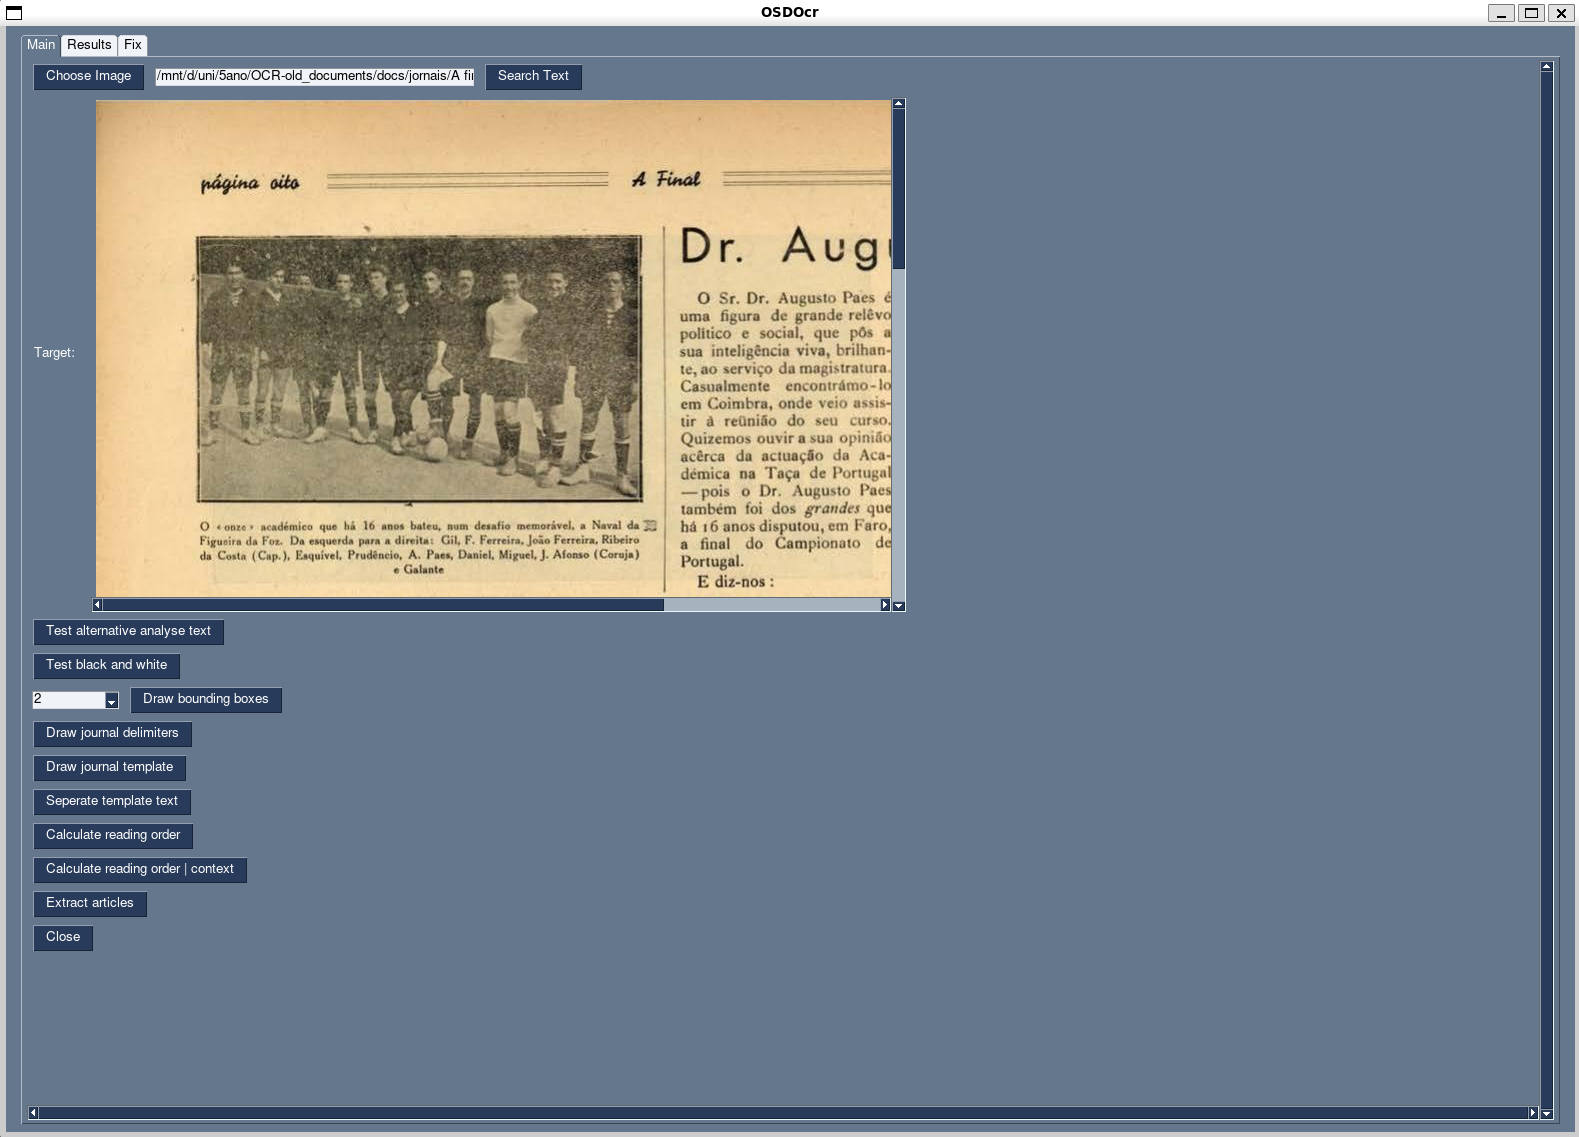
\includegraphics[width=1\textwidth]{images/implementacao/gui/gui_base.png}
    \caption{Interface gráfica simples}
    \label{fig:gui_base}
\end{figure}

\subsubsection{Visualização de bounding boxes}

\begin{figure}[H]
    \centering
    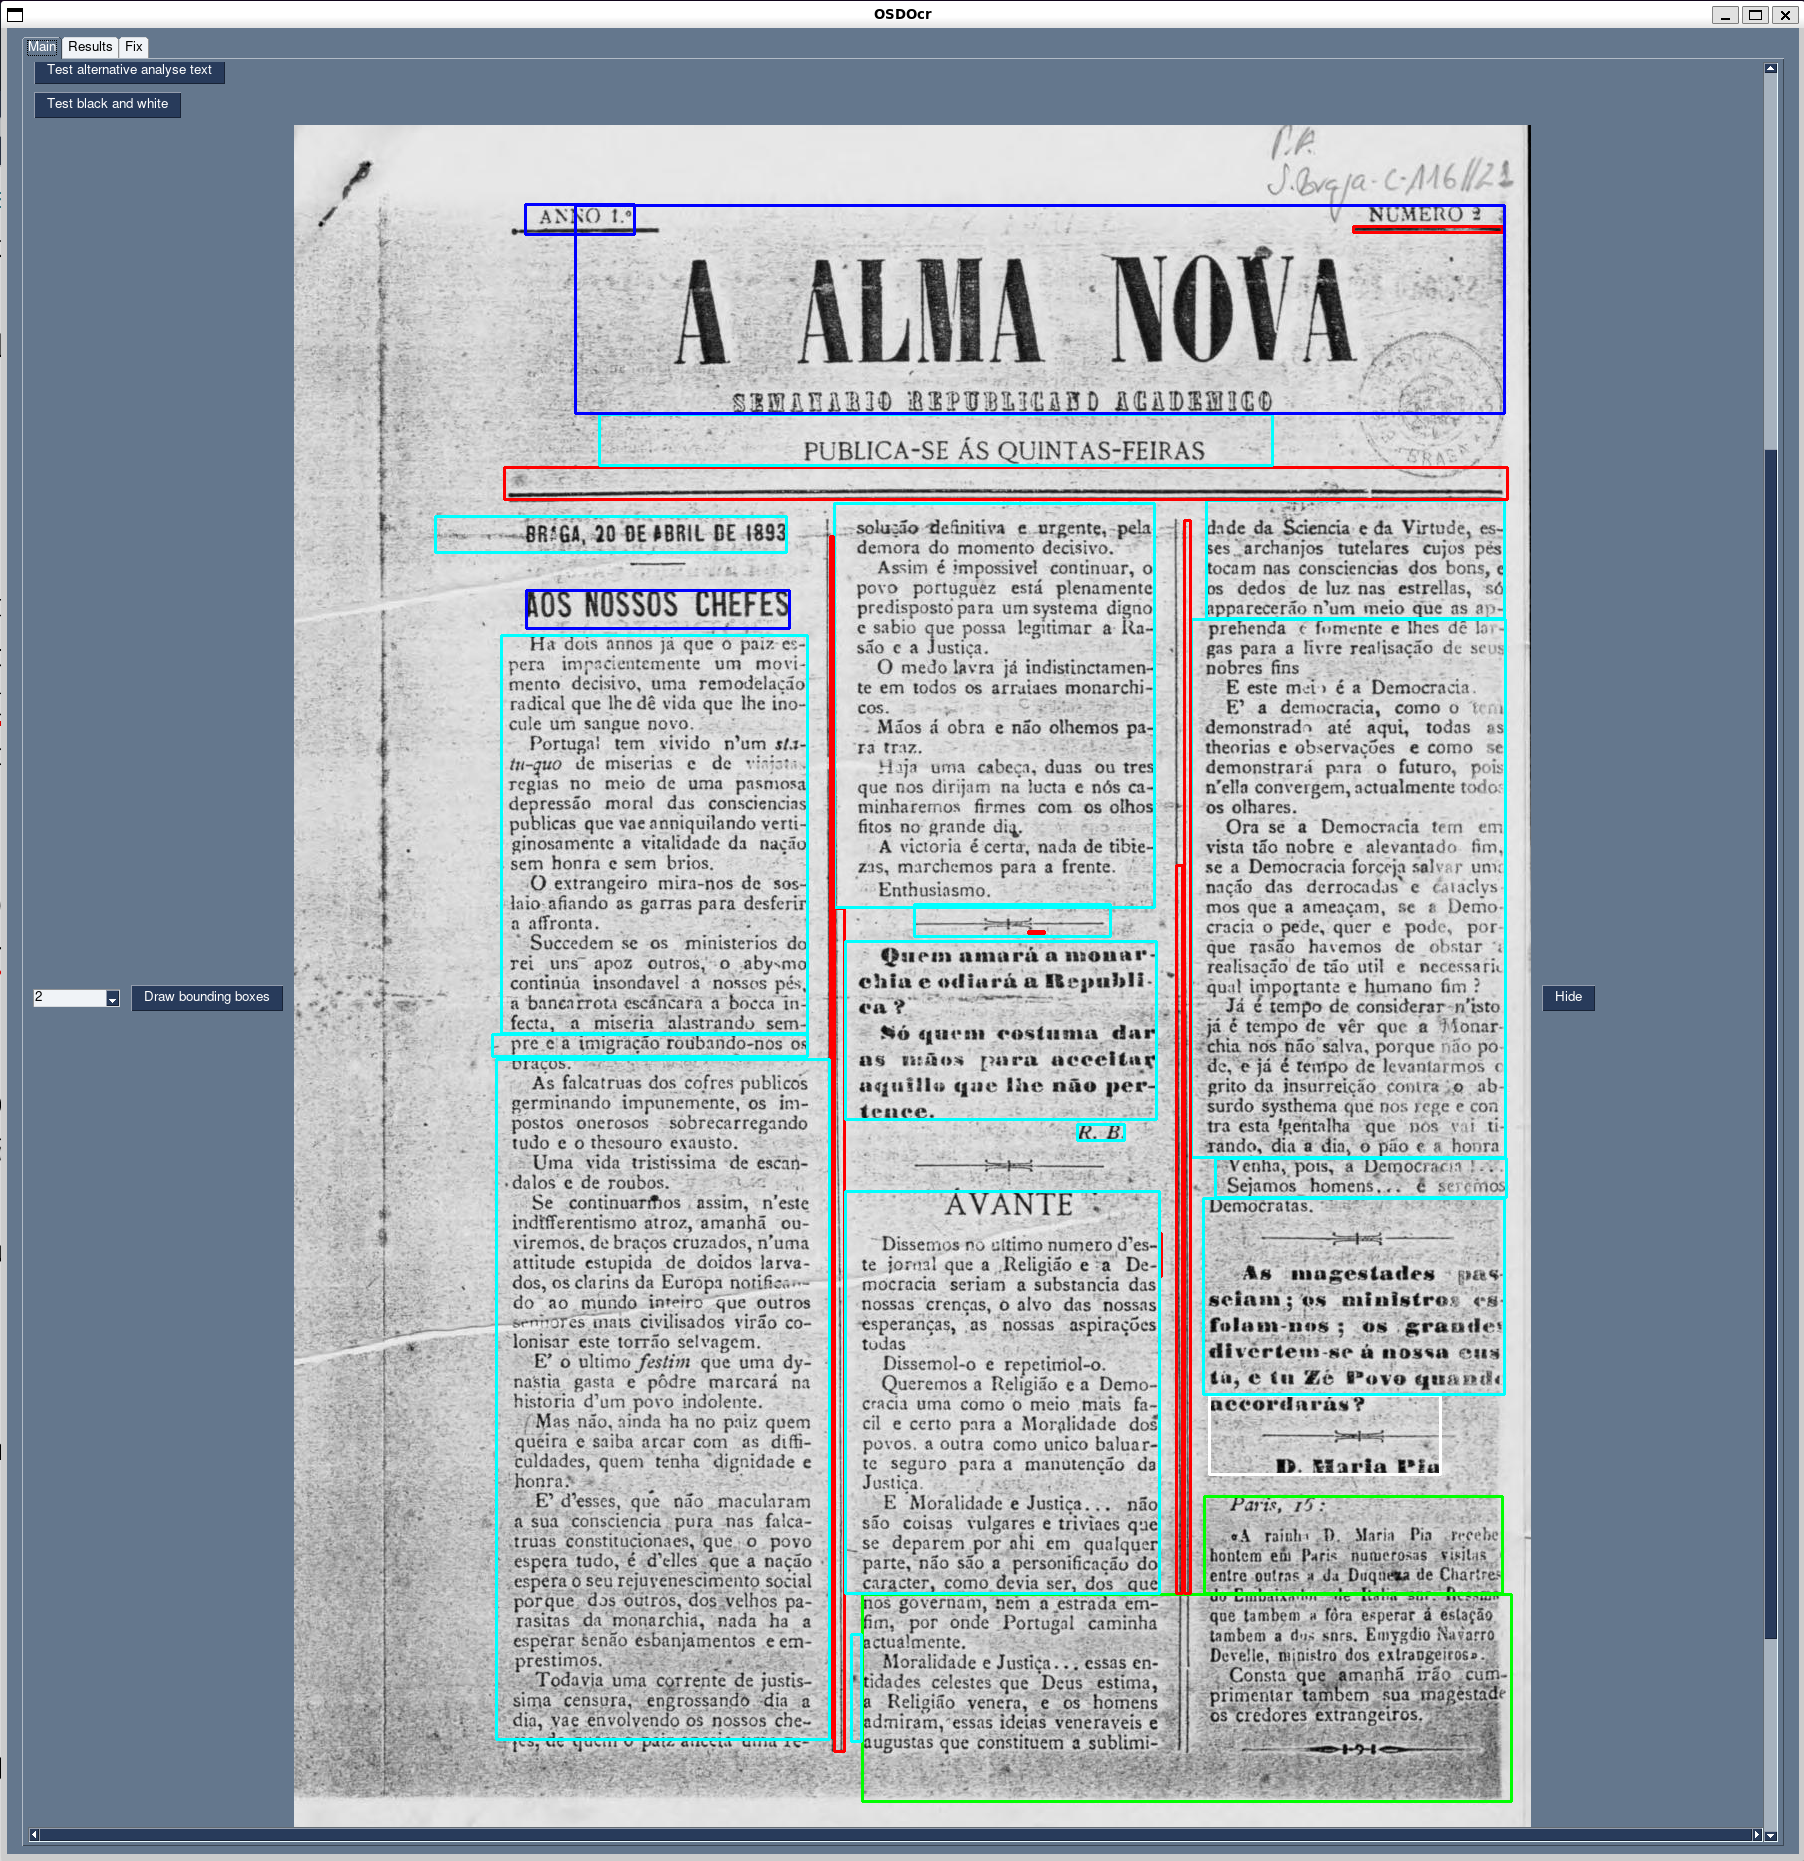
\includegraphics[width=1\textwidth]{images/implementacao/gui/gui_draw_bb.png}
    \caption{Visualização dos blocos resultantes de OCR}
    \label{fig:gui_draw_bb}
\end{figure}

A visualização de blocos dispõe também de coloração diferente para os blocos de acordo com a sua categorização. Blocos título estão a azul escuro, texto a azul claro, delimitadores a vermelho, legendas a branco e o resto - imagens, outros - a verde.

\subsubsection{Cálculo de template de jornal}

\begin{figure}[H]
    \centering
    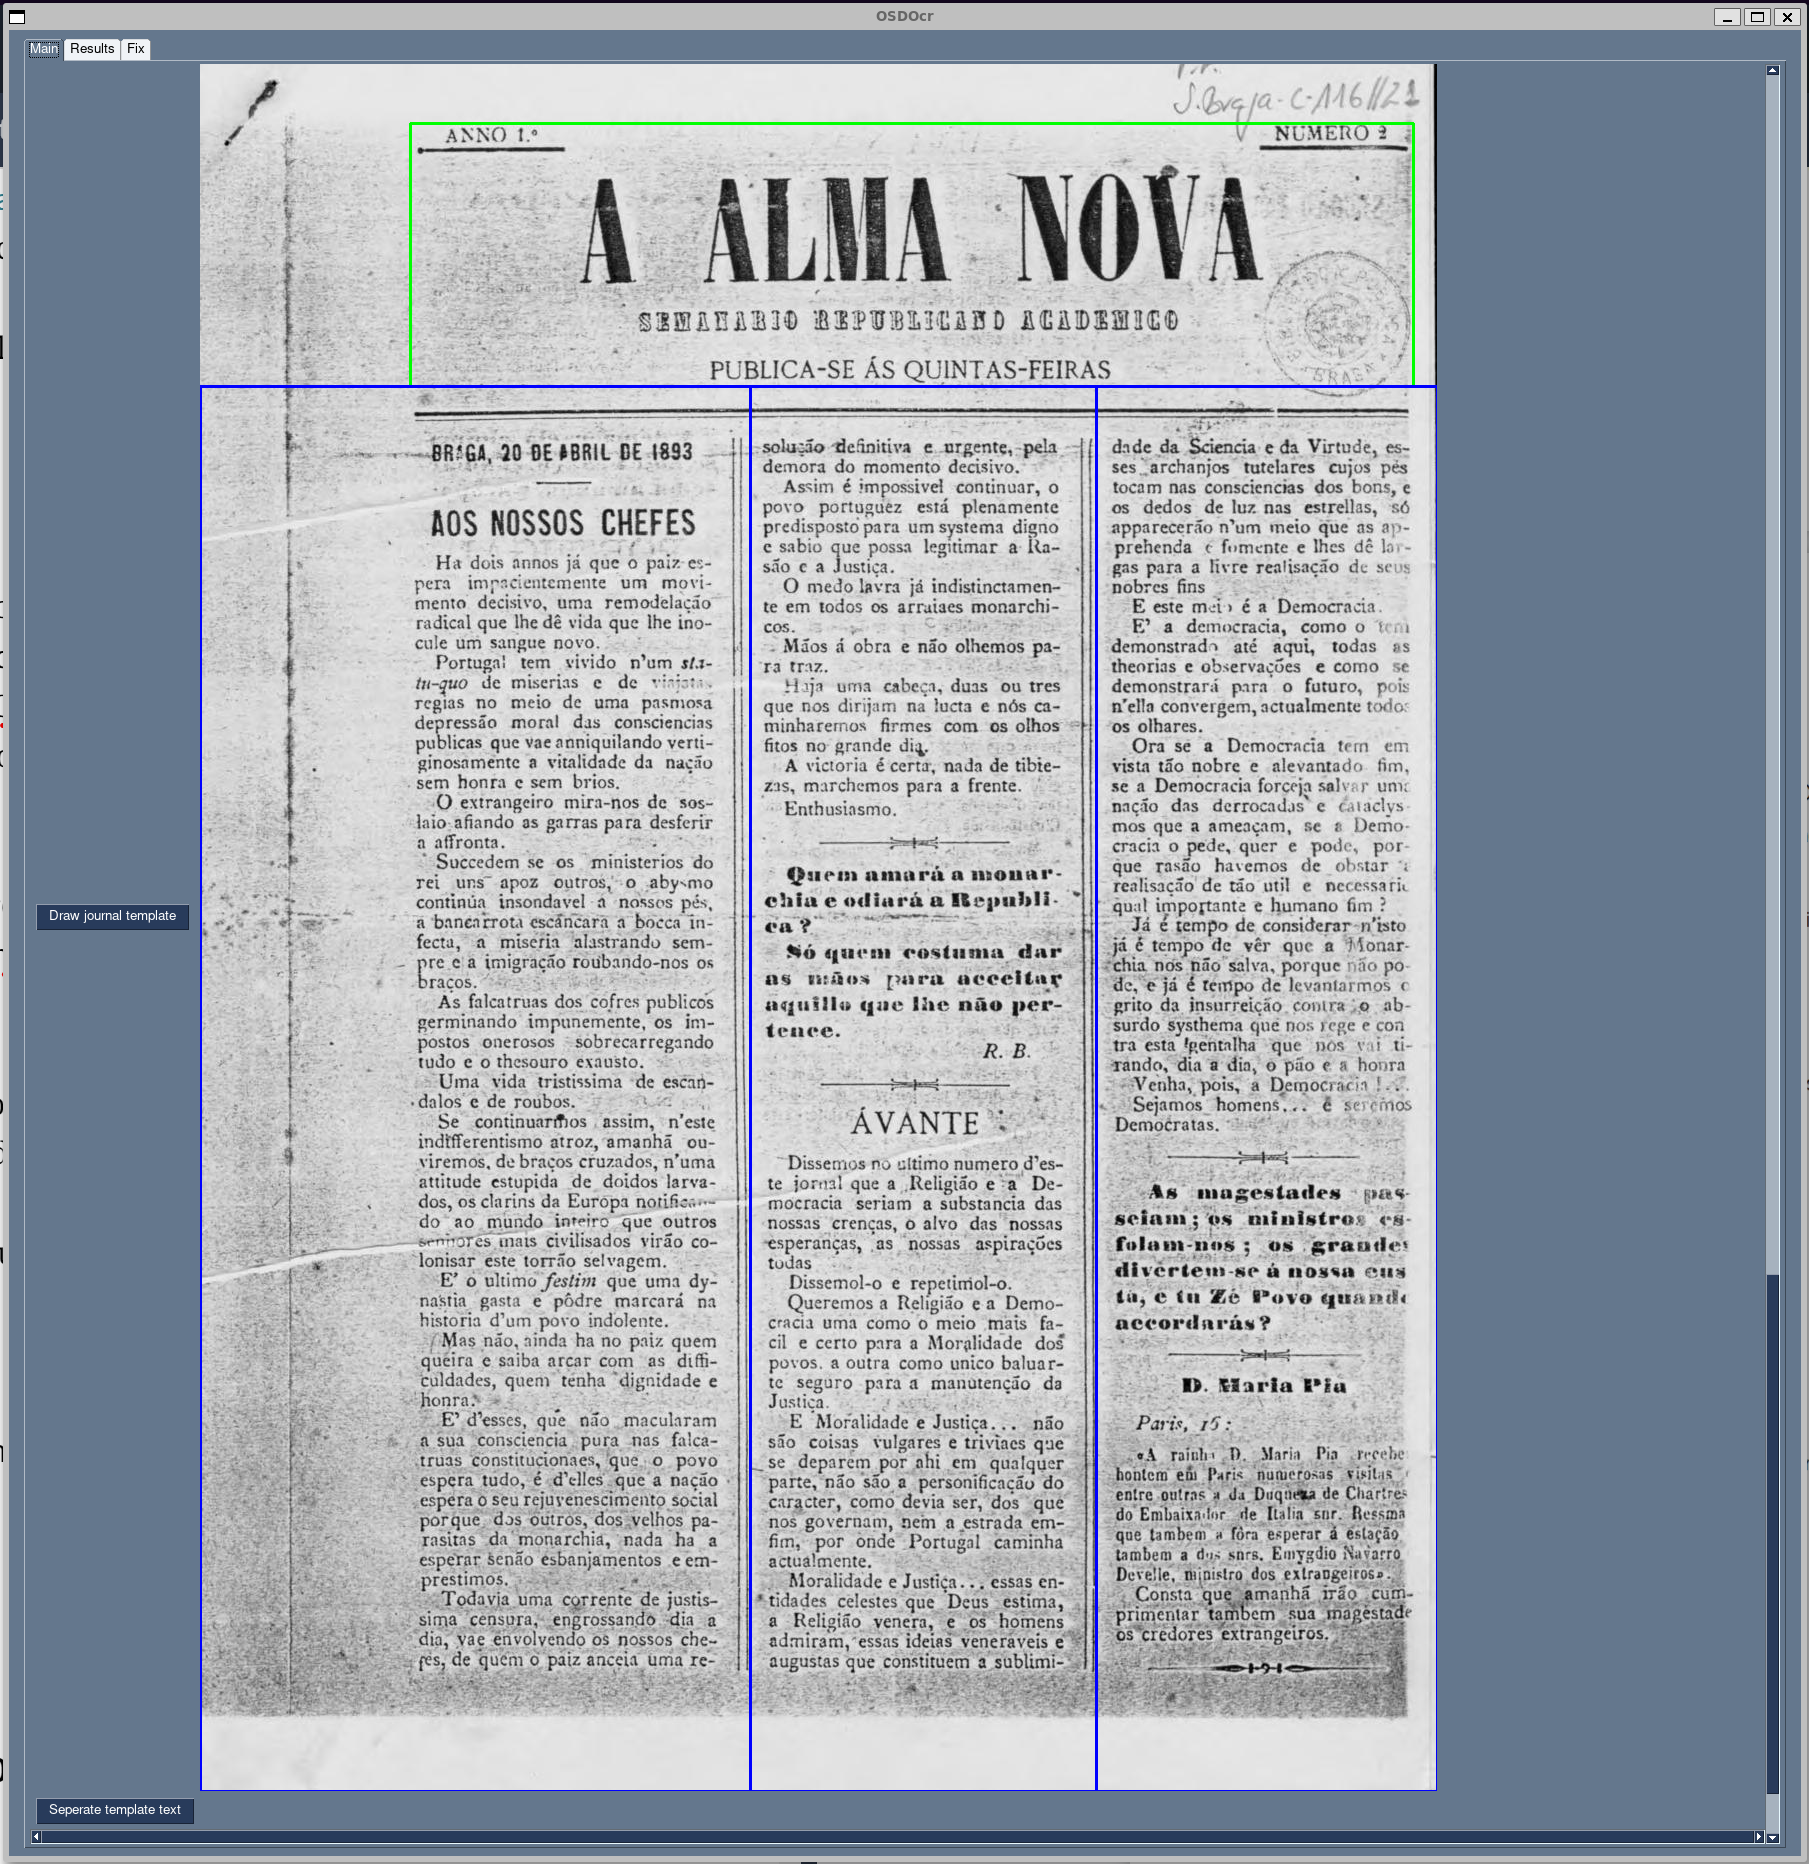
\includegraphics[width=1\textwidth]{images/implementacao/gui/gui_draw_template.png}
    \caption{Visualização do cálculo do template de jornal}
    \label{fig:gui_draw_template}
\end{figure}

O cálculo de template é feito através da deteção e análise dos delimitadores dos resultados OCR. Áreas são depois calculadas de acordo com estes delimitadores e, como se pode ver no caso do Header (caixa a verde) da imagem \ref{fig:gui_draw_template}, a área é ajustada de acordo com as caixas com texto da respetiva área.

\subsubsection{Extração de artigos}

\begin{figure}[H]
    \centering
    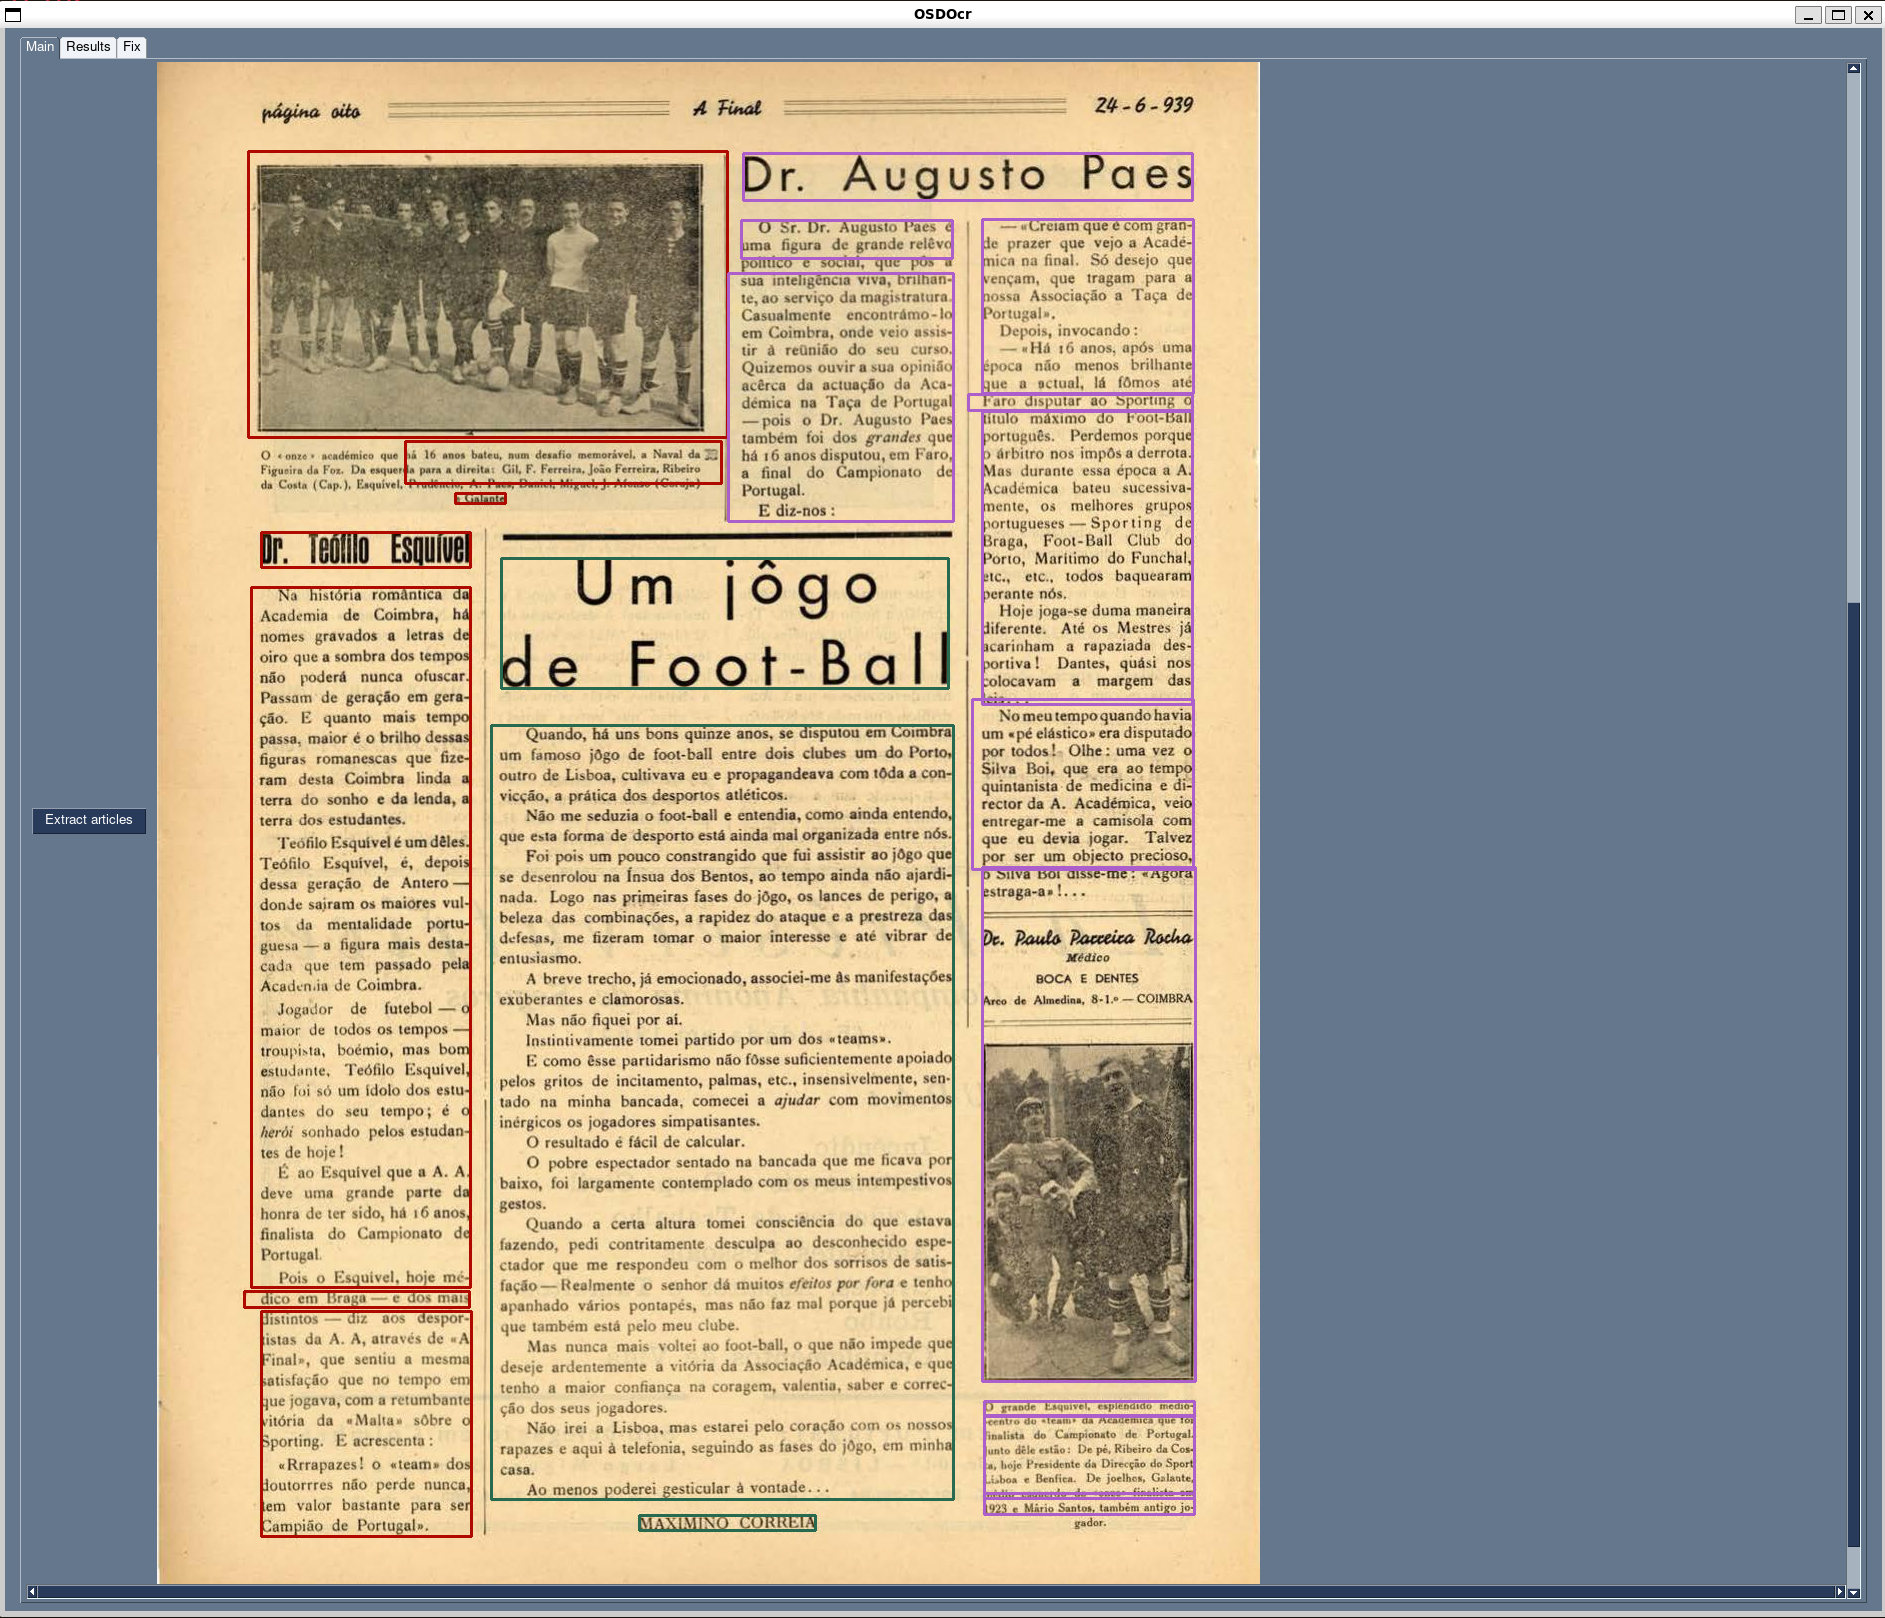
\includegraphics[width=1\textwidth]{images/implementacao/gui/gui_draw_articles.png}
    \caption{Visualização dos artigos extraídos}
    \label{fig:gui_draw_article}
\end{figure}

Neste caso, os artigos são calculados e posteriormente escolhidas cores distintas para realçar cada um destes. Os artigos são representados pelo conjunto de blocos que foram agrupados como sendo um dado artigo.

\subsubsection{Limpeza de bounding boxes}

\begin{figure}[H]
    \centering
    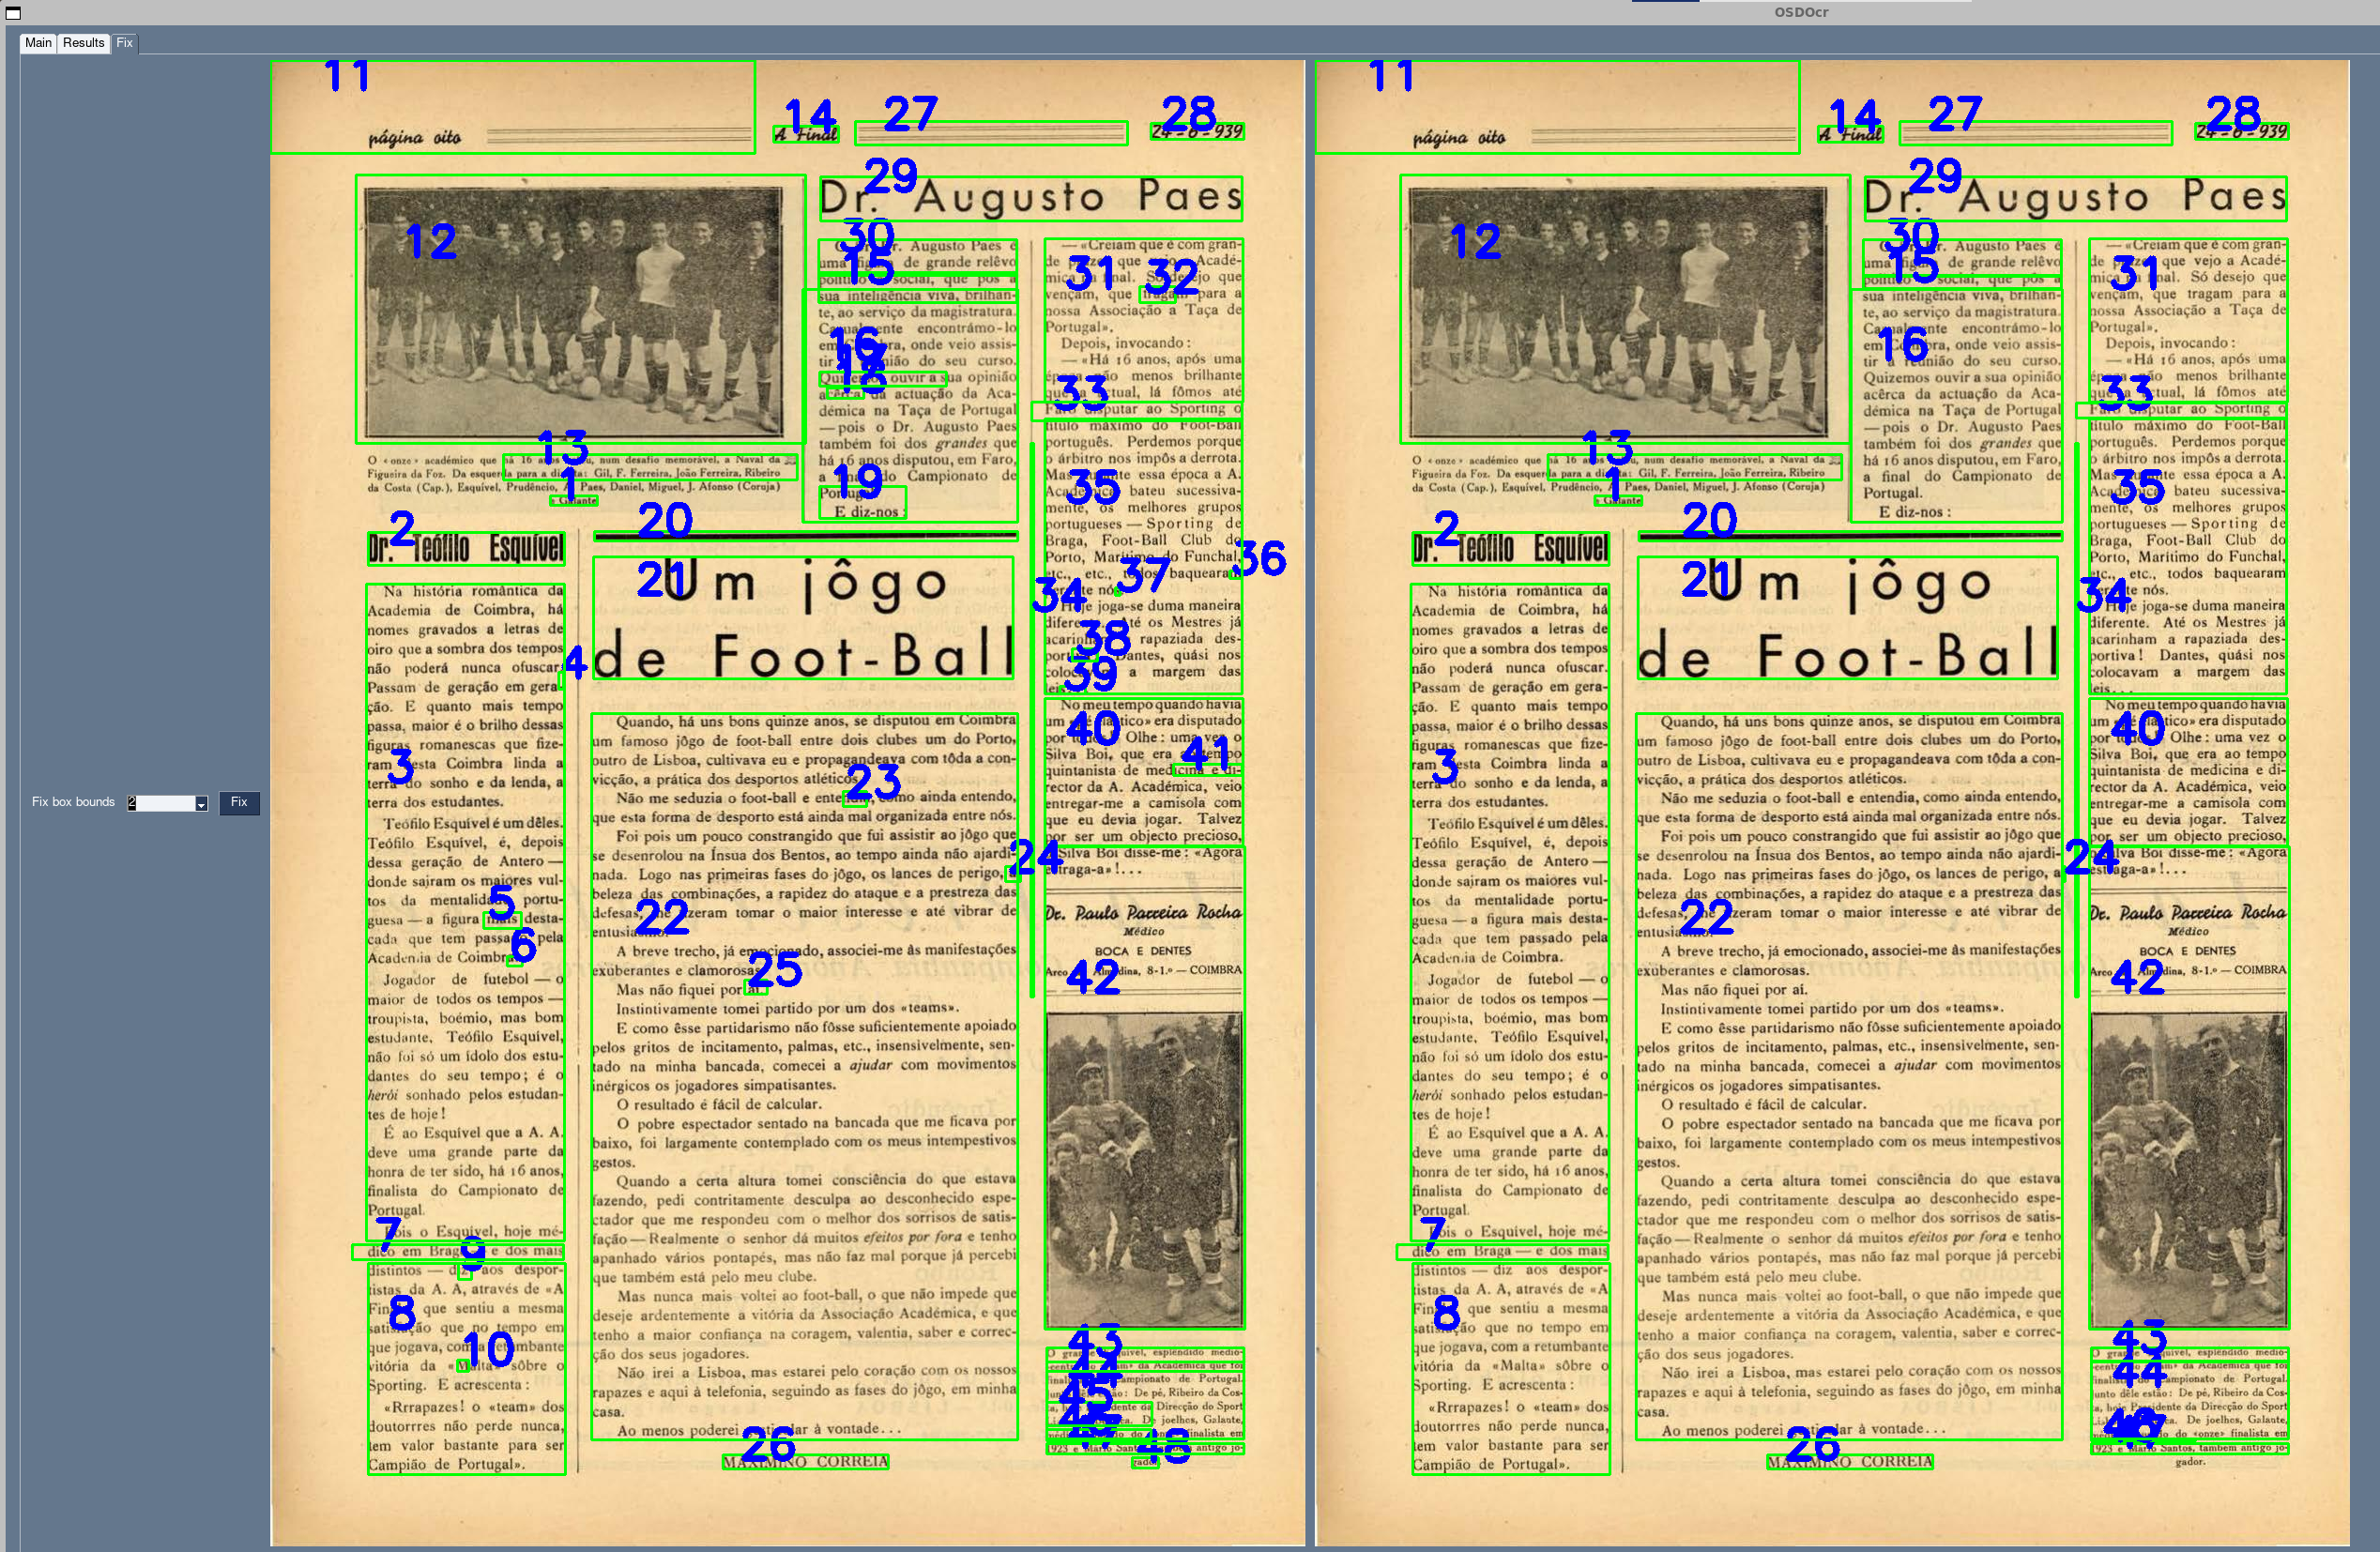
\includegraphics[width=1\textwidth]{images/implementacao/gui/gui_fix_blocks.png}
    \caption{Visualização da limpeza de blocos}
    \label{fig:gui_fix_bb}
\end{figure}

Para facilitar a deteção das diferenças entre o antes e depois da limpeza, os dois estados são postos lado a lado e os blocos são identificados, mantendo a mesma identificação após a limpeza. 




\section{Categorização de blocos}
\label{categorizacao_blocos}

Como verificado em vários dos estudos no estado da arte, por vezes, para realizar a segmentação correta dos documentos, é necessário considerar mais do que as posições relativas entre as diferentes caixas de texto. Por isto, um categorização destas caixas através de uma análise das suas características, permite o armazenamento de algum contexto sobre estas.

Atualmente, as caixas são categorizados em 1 destes tipos:

\begin{itemize}
    \item \textbf{Delimitador} : Caixa vazia (sem texto) e que cumpre a regra:

        $box.width >= 4*box.height \vee box.height >= 4*box.width$
        \item \textbf{Texto} : Tamanho médio do texto é do tamanho médio do documento, com uma margem de 30\%. Necessita uma análise de texto do documento.
        \item  \textbf{Título} : Tamanho médio acima do tamanho médio do documento.
        \item \textbf{Legenda} : Tamanho médio abaixo do tamanho médio do documento.
        \item \textbf{Outro} : Para as caixas que não correspondem a nenhum dos outros casos. Método provisório para categorizar imagens e outros elementos sem texto.
\end{itemize}

    Além disso, para as caixas com texto, verificam-se algumas características deste, nomeadamente:
    \begin{itemize}
        \item \textbf{Texto iniciado} : Se a primeira letra for maiúscula.
        \item \textbf{Texto não terminado} : Se não tiver terminado com uma pontuação de fim de frase.
    \end{itemize}

A figura \ref{fig:gui_draw_bb} apresenta os blocos categorizados através deste algoritmo.

Trabalho futuro neste procedimento, consistirá em, além das melhorias na categorização já realizada, possibilitar a identificação de outras entidades como imagens, anúncios ou tabelas.






\section{Ordenação de blocos}
\label{ordenacao_blocos}

Como observado no estado da arte, documentos complexos, como são exemplo jornais, necessitam um maior cuidado na reconstrução do seu conteúdo em comparação com documentos mais simples como um livro regular. Isto deve-se ao facto dos elementos de texto que o compõe nem sempre seguem uma ordem simples (cima para baixo e esquerda para a direita), sendo muitas vezes irregulares e dependentes de alguma forma de contexto, seja delimitadores, imagens ou mesmo o conteúdo do texto.

Deste modo, o cálculo da ordem de leitura dos resultados de OCR é uma das tarefas primárias deste projeto.

Atualmente, a implementação da ordenação de blocos, segue métodos de heurísticas utilizando grafos. Tal permite, como em casos observados em trabalhos relacionados na secção  \ref{sec_trab_relacionado}, a combinação de ordenação tendo em conta a posição dos blocos e também, pelo peso entre os nodos, correspondente a um nível de atração calculado tendo em conta o contexto.

Assumindo um pós processamento de limpeza dos blocos, começa-se com a criação de um grafo de ligação entre os blocos. As ligações criadas entre os blocos neste ponto seguem apenas regras simples de posição relativa, i.e. um bloco apenas pode ter como filhos blocos, adjacentes, por baixo de si ou diretamente à sua direita.

Com o grafo criado, segue-se o cálculo dos pesos. Estes tomam em conta tanto a posição relativa dos blocos, sendo que por norma um bloco tem tendência a ser seguido por um bloco abaixo, mas também o contexto, permitindo corrigir este preconceito quando evidente. O contexto atualmente considerado é:
\begin{itemize}
    \item \textbf{Categoria dos blocos} : certos tipos de blocos são mais atraídos por tipos específicos. Ex.: imagem e legenda; título e bloco não título.
    \item \textbf{Características de blocos de texto} : caso um bloco de texto não esteja acabado, então ele é naturalmente mais atraído para blocos de texto que não estejam iniciados.
\end{itemize}

Procede-se com uma poda das ligações de filhos para pais de forma a remover ligações com atração muito baixa e assim reduzir dependências dos nodos. A remoção é realizada quando entre dois nodos existem ligações que tenham peso duas ou mais vezes maior do que as outras.

Por último, o grafo é ordenado pelo caminho de maior custo. Tem-se aqui em conta que o próximo nodo escolhido para ordenar não pode ter dependências ativas, i.e. todos os seus potenciais pais têm de já ter sido escolhidos.

\begin{figure}[H]
    \hspace*{-4.5cm}
    \includegraphics[width=1.5\textwidth]{images/implementacao/algoritmos/comparacao_ordem_leitura.png}
    \caption{Comparação de ordens de leitura: (a) ordem correta; (b) ordem do Tesseract; (c) ordem do algoritmo implementado}
    \label{fig:comp_reading_order}
\end{figure}

Como se observa na imagem \ref{fig:comp_reading_order}, para o exemplo desta página de jornal, a ordem de leitura calculada pelo algoritmo, embora com alguns erros, assemelha-se significativamente mais À correta do que a fornecida pelo Tesseract.



Esta implementação ainda pode ser denotada como \textit{naive} visto ainda incluir pouco contexto na sua lógica. Outras implementações terão de ser experimentadas e comparadas no futuro.

No entanto, este ponto de partida já permite uma extração simples de artigos. Tendo em conta a ordem de leitura e, assumindo que um artigo é sempre inicializado por um título, podemos cortar a sequência ordenada das caixas pelos seus títulos e assim dividir em artigos. A figura \ref{fig:gui_draw_article} é um exemplo disto. É de notar no entanto, que uma posterior ordenação destes artigos poderia ser realizada.
